% Chapter 4: Thiết kế CSDL Cấp độ 1 & 2: Mô hình Ý niệm và Logic

Thiết kế cơ sở dữ liệu là trục trung tâm của đồ án. Để đạt được chất lượng học thuật và thực tiễn kỹ thuật ở mức xuất sắc nhất, quy trình thiết kế được phân tách rạch ròi thành 3 cấp độ trừu tượng: \textbf{Mô hình Ý niệm (Conceptual Design)} $\rightarrow$ \textbf{Mô hình Logic (Logical Design)} $\rightarrow$ \textbf{Mô hình Vật lý (Physical Design)}. Chương này trình bày chi tiết hai cấp độ đầu tiên: từ các khái niệm nghiệp vụ thuần túy đến mô hình quan hệ được chuẩn hóa chặt chẽ theo dạng chuẩn 3 (3NF).

% ----------------------------------------------------------------------
\section{Phương pháp luận và Phân định 3 Cấp độ Trừu tượng}
\label{s:c4_methodology}

\paragraph{Artifact Synchronization}
The Markdown specification and this LaTeX chapter describe the same conceptual
contract. Canonical entity names, relationship cardinalities, business rules,
and decision boundaries must remain identical across both artifacts; LaTeX may
add presentation structure but must not introduce a different model.

Một trong những sai lầm phổ biến nhất trong thiết kế cơ sở dữ liệu là ``vẽ 3 sơ đồ ERD gần giống nhau'', làm mất đi bản chất của từng giai đoạn. Dự án phân định rạch ròi ranh giới trừu tượng như sau:

\begin{enumerate}
    \item \textbf{Cấp độ 1 -- Thiết kế Ý niệm (Conceptual Model)}: Trả lời câu hỏi \textit{``Thế giới thực có những đối tượng nghiệp vụ nào và mối quan hệ giữa chúng là gì?''}. Mô hình hoàn toàn độc lập với mọi hệ quản trị CSDL, không chứa kiểu dữ liệu kỹ thuật, chỉ tập trung vào bản số (\textit{cardinality}), tính tùy chọn (\textit{optionality}) và xuất xứ dữ liệu (\textit{provenance}).
    \item \textbf{Cấp độ 2 -- Thiết kế Logic (Logical Model)}: Trả lời câu hỏi \textit{``Dữ liệu được tổ chức thành các bảng quan hệ như thế nào?''}. Giai đoạn này chuyển đổi thực thể thành các quan hệ (\textit{relations}), giải quyết triệt để quan hệ Nhiều-Nhiều ($N:M$), xác định khóa chính (PK), khóa ngoại (FK), khóa thay thế (Alternate Keys), thực hiện chuẩn hóa đến dạng chuẩn 3 (3NF) và xây dựng từ điển dữ liệu logic.
    \item \textbf{Cấp độ 3 -- Thiết kế Vật lý (Physical Model)}: Trả lời câu hỏi \textit{``Cấu trúc dữ liệu được cài đặt cụ thể trên DBMS mục tiêu như thế nào?''}. Lựa chọn kiểu dữ liệu chính xác trên Microsoft SQL Server, thiết lập ràng buộc (CHECK, UNIQUE, FK actions), chiến lược đánh chỉ mục (Index) và lập trình CSDL (Views, Stored Procedures, Triggers).
\end{enumerate}

\paragraph{Quy ước Tên Thực thể Chuẩn}
Trong toàn bộ tài liệu TV4, tên thực thể được chuẩn hóa như sau: \\texttt{ParticipantProfile} là thực thể dữ liệu của thí sinh; ``verification'' là quy trình còn \\texttt{VerificationCase} là hồ sơ thẩm định; \\texttt{AwardDefinition} là cơ cấu giải và \\texttt{AwardAssignment} là việc gán giải; ``digital archive'' là năng lực nghiệp vụ còn \\texttt{ArchiveItem} là bản ghi lịch sử. Giám khảo là \\texttt{UserAccount} mang vai trò Judge, không tạo thêm thực thể Judge.
Tên canonical phải được giữ nguyên trong ERD ý niệm, caption, bảng truy vết và các tham chiếu sang mô hình logic; nhãn tiếng Việt chỉ dùng để giải thích, không thay thế tên định danh chuẩn.

% ----------------------------------------------------------------------
\section{Thiết kế Cấp độ 1: Danh mục Thực thể Ý niệm (Entity Inventory)}
\label{s:c4_conceptual_entities}

Mô hình ý niệm bao phủ trọn vẹn chuỗi giá trị từ tài khoản người dùng đến lưu trữ di sản số:
\begin{equation*}
\begin{split}
\text{UserAccount/Role} \rightarrow \text{ParticipantProfile} \rightarrow \text{Registration} \rightarrow \text{FilmRoll} \\
\rightarrow \text{FilmFrame} \rightarrow \text{Submission} \rightarrow \text{VerificationCase} \rightarrow \text{JudgingRound/Evaluation} \\
\rightarrow \text{Result/AwardAssignment} \rightarrow \text{ArchiveItem} \rightarrow \text{AuditLog}
\end{split}
\end{equation*}

Danh mục chi tiết 32 thực thể ý niệm và vai trò tương ứng được tổng hợp trong Bảng~\ref{tab:c4_entity_inventory}:

\begin{table}[!ht]
\centering
\caption{Danh mục 32 thực thể ý niệm và logic trong hệ thống}
\label{tab:c4_entity_inventory}
\scriptsize
\begin{tabularx}{\textwidth}{>{\bfseries}p{3.2cm}p{4.8cm}>{\raggedright\arraybackslash}X}
\toprule
\textbf{Thực thể Ý niệm} & \textbf{Ý nghĩa nghiệp vụ trong thế giới thực} & \textbf{Lý do cần ở mức ý niệm} \\
\midrule
\textbf{UserAccount} & Danh tính người dùng truy cập nền tảng. & Tách danh tính khỏi nghiệp vụ. \\
\textbf{Role} & Vai trò trách nhiệm (Admin, Organizer, Judge, Participant). & Chuẩn hóa từ vựng phân quyền. \\
\textbf{UserRole} & Phân công vai trò cho tài khoản. & Biểu diễn quan hệ N:M User--Role. \\
\textbf{ParticipantProfile} & Hồ sơ chi tiết của thí sinh. & Lưu dữ liệu nghiệp vụ riêng của thí sinh. \\
\textbf{Contest} & Sự kiện thi có thể lệ và thời gian. & Neo toàn bộ vòng đời cuộc thi. \\
\textbf{ContestCategory} & Hạng mục chuyên môn trong cuộc thi. & Phân định điều kiện, chấm và kết quả theo hạng mục. \\
\textbf{Registration} & Đơn đăng ký của thí sinh vào cuộc thi. & Ghi nhận giao dịch tham gia trước khi nộp bài. \\
\textbf{FilmStock} & Danh mục dòng phim. & Bảo toàn xuất xứ kỹ thuật của cuộn phim. \\
\textbf{Camera} & Danh mục thân máy ảnh. & Nhận diện thiết bị chụp của frame. \\
\textbf{Lens} & Danh mục ống kính. & Nhận diện thiết bị quang học của frame. \\
\textbf{Lab} & Danh mục phòng lab tráng phim. & Bảo toàn xuất xứ xử lý cuộn phim. \\
\textbf{FilmRoll} & Cuộn phim vật lý của thí sinh. & Nhóm các frame và metadata phim. \\
\textbf{FilmFrame} & Khung hình đơn trên cuộn phim. & Là nguồn vật lý của bài dự thi. \\
\textbf{Submission} & Tác phẩm gắn frame với đăng ký và hạng mục. & Đối tượng được thẩm định, chấm và xếp hạng. \\
\textbf{VerificationCase} & Hồ sơ thẩm định bài dự thi. & Tách quyết định con người khỏi submission. \\
\textbf{AIAnalysisResult} & Kết quả phân tích AI mang tính tư vấn. & Lưu bằng chứng AI nhưng không thay quyết định người. \\
\textbf{JudgingRound} & Vòng chấm trong một hạng mục. & Hỗ trợ chấm nhiều vòng. \\
\textbf{JudgeAssignment} & Phân công giám khảo vào vòng chấm. & Xác định phạm vi công việc. \\
\textbf{ScoringCriterion} & Tiêu chí, trọng số và thang điểm. & Định nghĩa cách đánh giá theo vòng. \\
\textbf{Evaluation} & Phiếu đánh giá của một giám khảo. & Ghi nhận sự kiện chấm điểm nguyên tử. \\
\textbf{EvaluationScore} & Điểm theo từng tiêu chí. & Giải quyết quan hệ N:M Evaluation--Criterion. \\
\textbf{Result} & Kết quả xếp hạng chính thức. & Bảo toàn kết quả cuối cùng. \\
\textbf{AwardDefinition} & Định nghĩa cơ cấu giải thưởng. & Tách cấu hình giải khỏi người nhận giải. \\
\textbf{AwardAssignment} & Gán giải cho kết quả chung cuộc. & Ghi nhận kết quả trao giải. \\
\textbf{ArchiveItem} & Bản chụp bất biến của kết quả được lưu trữ. & Bảo toàn lịch sử khi dữ liệu sống thay đổi. \\
\textbf{AuditLog} & Nhật ký thay đổi nghiệp vụ quan trọng. & Bảo đảm truy vết và trách nhiệm. \\
\textbf{ContestTemplate} & Mẫu cấu hình cuộc thi tái sử dụng. & Cho phép nhân bản nhanh cấu hình cuộc thi mới. \\
\textbf{TemplateCategory} & Hạng mục mẫu trong template. & Khung phân loại chuyên môn tái sử dụng. \\
\textbf{TemplateJudgingRound} & Vòng chấm thi mẫu trong template. & Khung vòng chấm định nghĩa sẵn. \\
\textbf{TemplateScoringCriterion} & Tiêu chí chấm điểm mẫu trong template. & Khung thang điểm và trọng số mẫu. \\
\textbf{TemplateAwardDefinition} & Cơ cấu giải thưởng mẫu trong template. & Khung giải thưởng mẫu cho hạng mục. \\
\textbf{AssetMetadata} & Siêu dữ liệu số hóa có cấu trúc và bằng chứng QC. & Quản lý MIME, kích thước, SHA-256, máy scan và QC. \\
\bottomrule
\end{tabularx}
\end{table}

\subsection{Kiểm tra Độ đầy đủ Danh mục Thực thể}
Danh mục thực thể bao phủ đầy đủ các năng lực nghiệp vụ cốt lõi mà không tạo
thêm thực thể Judge trùng với tài khoản người dùng:
\begin{itemize}
    \item \textbf{Danh tính và RBAC}: \texttt{UserAccount}, \texttt{Role}, \texttt{UserRole}, \texttt{ParticipantProfile}.
    \item \textbf{Mẫu cấu hình tái sử dụng}: \texttt{ContestTemplate}, \texttt{TemplateCategory}, \texttt{TemplateJudgingRound}, \texttt{TemplateScoringCriterion}, \texttt{TemplateAwardDefinition}.
    \item \textbf{Cấu hình cuộc thi}: \texttt{Contest}, \texttt{ContestCategory}, \texttt{JudgingRound}, \\ \texttt{ScoringCriterion}, \texttt{AwardDefinition}.
    \item \textbf{Đăng ký và xuất xứ}: \texttt{Registration}, \texttt{FilmStock}, \texttt{Camera}, \texttt{Lens}, \texttt{Lab}, \texttt{FilmRoll}, \texttt{FilmFrame}, \texttt{AssetMetadata}.
    \item \textbf{Nộp bài và thẩm định}: \texttt{Submission}, \texttt{VerificationCase}, \\ \texttt{AIAnalysisResult}.
    \item \textbf{Chấm thi}: \texttt{JudgeAssignment}, \texttt{Evaluation}, \texttt{EvaluationScore}.
    \item \textbf{Kết quả và bảo tồn lịch sử}: \texttt{Result}, \texttt{AwardAssignment}, \texttt{ArchiveItem}, \texttt{AuditLog}.
\end{itemize}

Mối quan hệ tổng thể giữa 32 thực thể được biểu diễn trực quan qua Sơ đồ Thực thể Liên kết Ý niệm trong Hình~\ref{fig:c4_conceptual_erd}:

\begin{figure}[!ht]
    \centering
    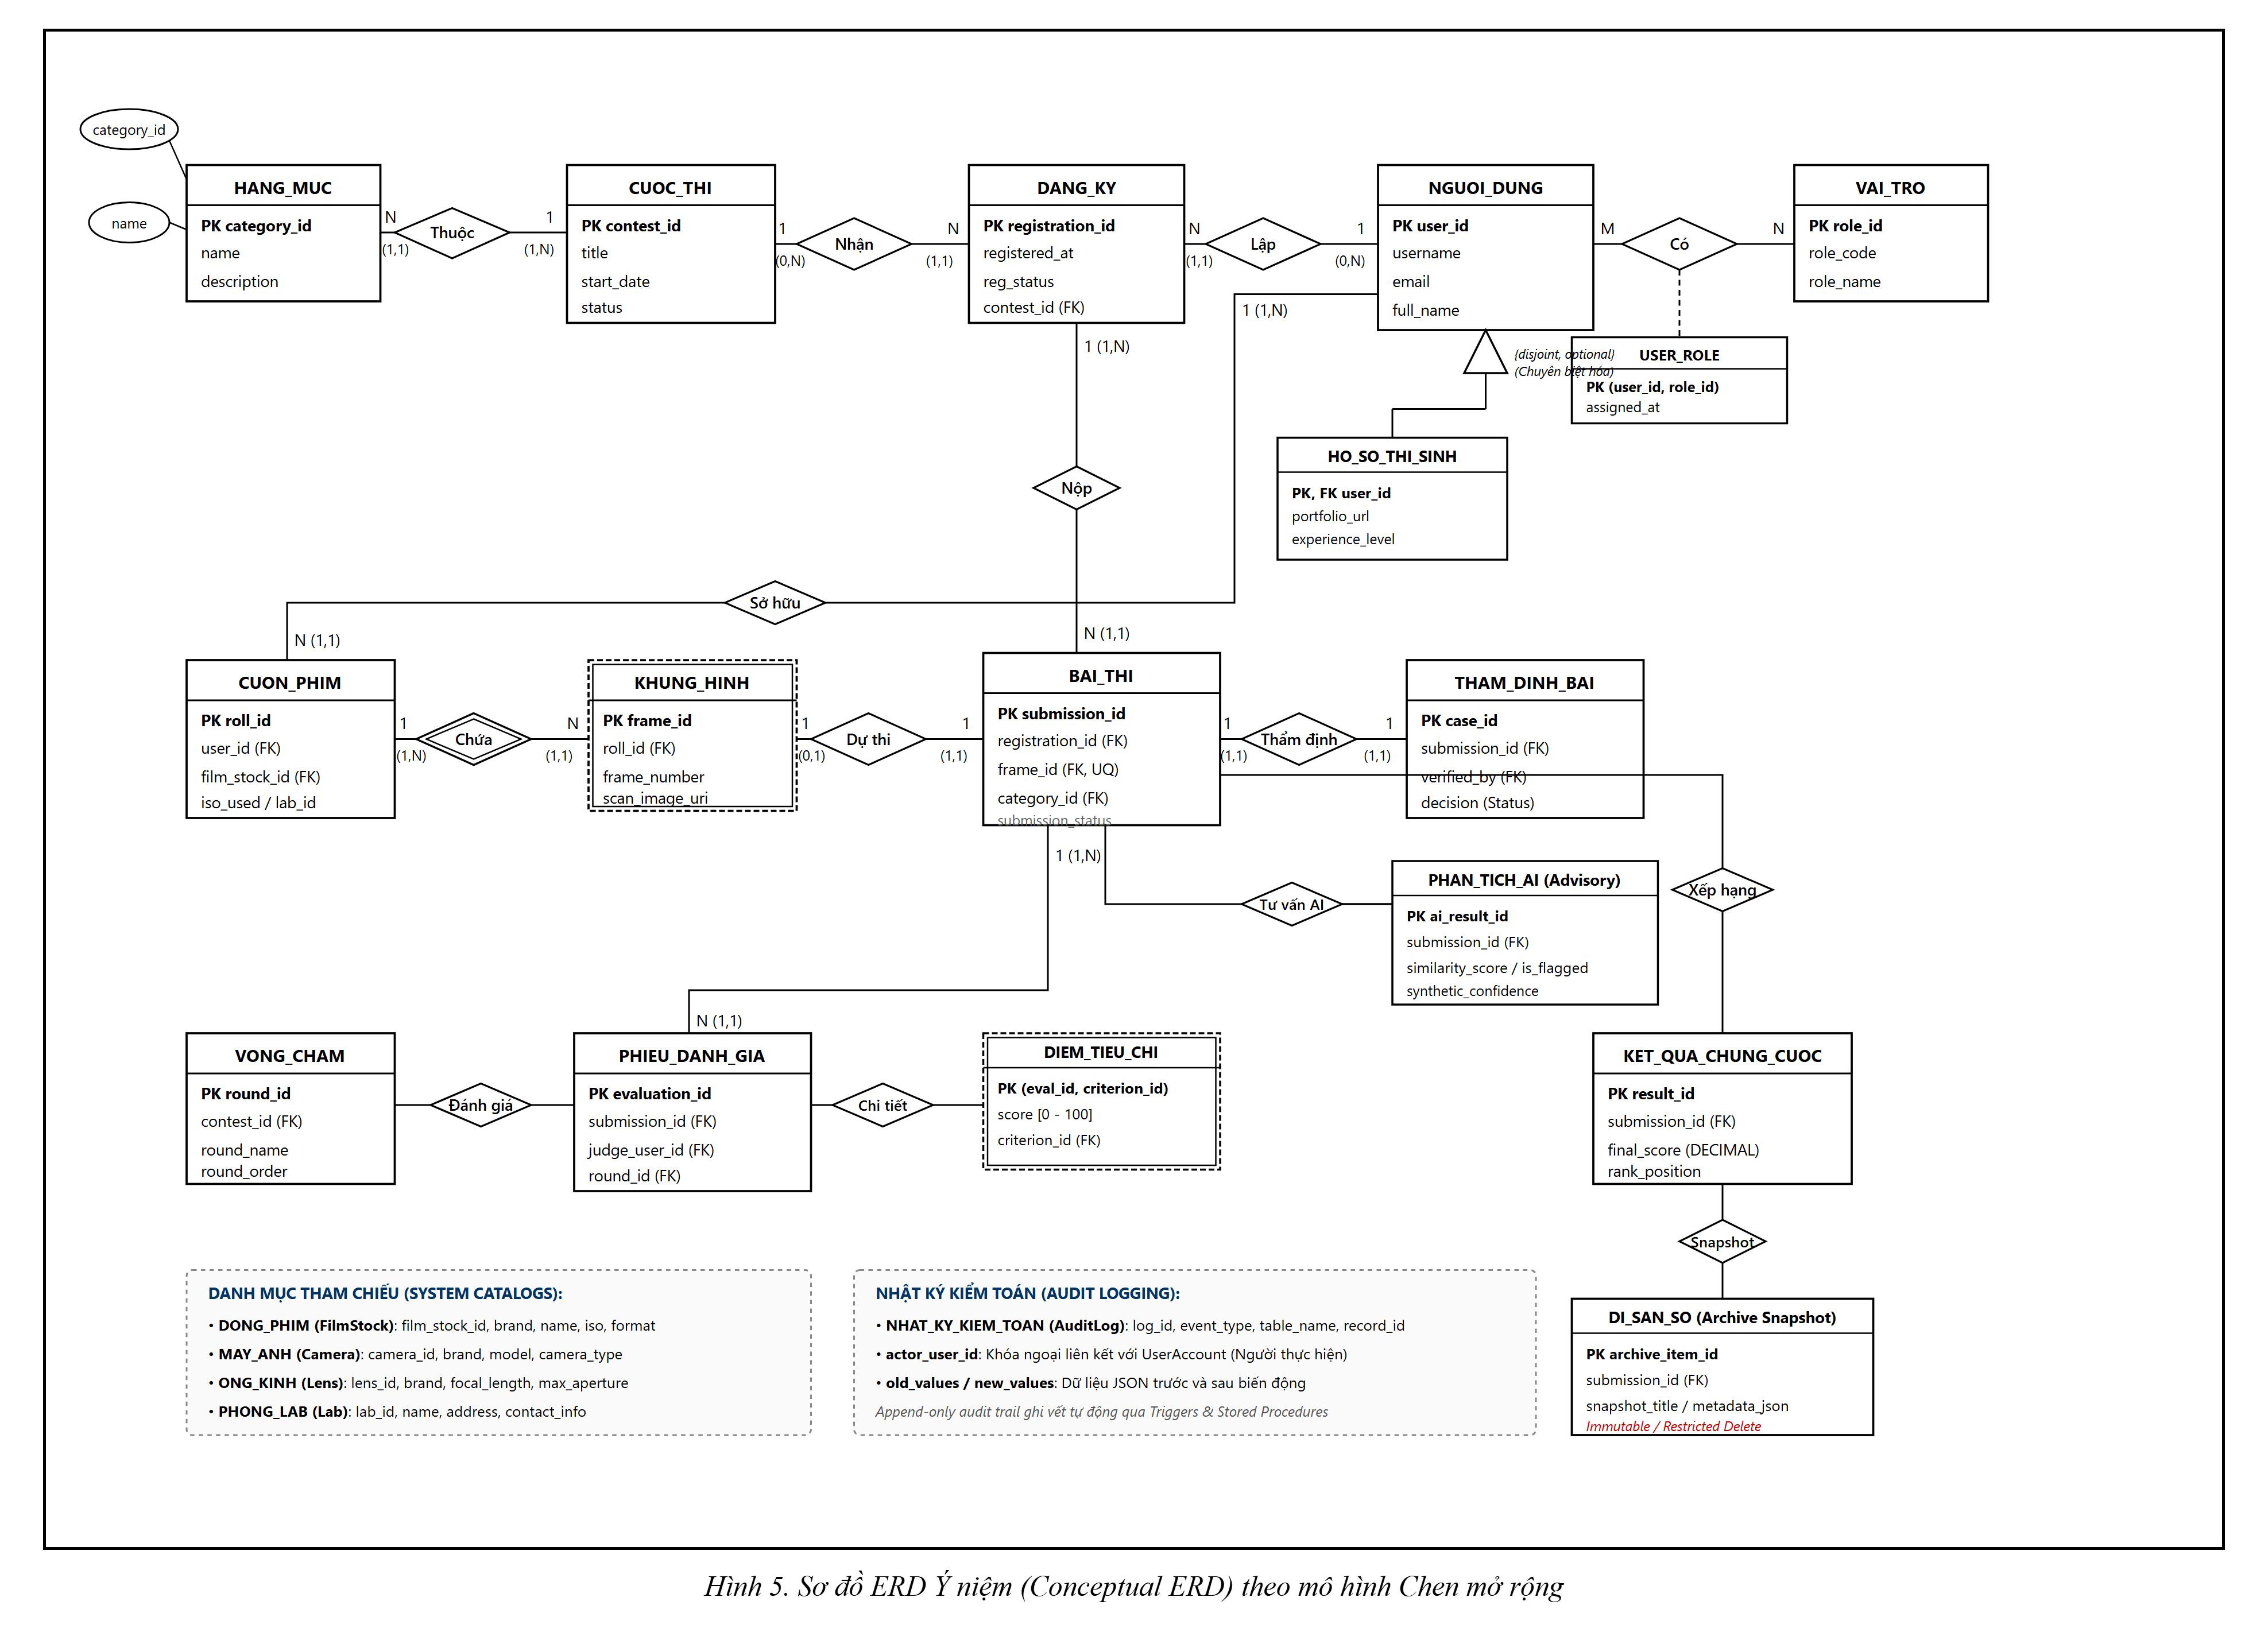
\includegraphics[width=\textwidth,keepaspectratio]{figures/fig_conceptual_erd.png}
    \caption{Sơ đồ Thực thể Liên kết Ý niệm (Conceptual ERD) chuẩn hóa 32 thực thể}
    \label{fig:c4_conceptual_erd}
\end{figure}

% ----------------------------------------------------------------------
\section{Bản số (Cardinality) và Ràng buộc Quan hệ Ý niệm}
\label{s:c4_cardinalities}

Mỗi mối quan hệ được xác lập bằng bản số chuẩn (\textit{Cardinality}):
\begin{itemize}
    \item \textbf{Phân hệ Quản trị Cuộc thi}:
    \begin{itemize}
        \item $\text{Contest } (1,1) \longleftrightarrow (1,N) \text{ ContestCategory}$: Mỗi cuộc thi bắt buộc có ít nhất một hạng mục chuyên môn (BR-O-001).
        \item $\text{Contest } (1,1) \longleftrightarrow (0,N) \text{ Registration}$: Cuộc thi tiếp nhận các đơn đăng ký từ thí sinh.
        \item $\text{Contest } (1,1) \longleftrightarrow (0,N) \text{ Submission}$: Cuộc thi là ngữ cảnh chứa các bài dự thi.
    \end{itemize}
    \item \textbf{Phân hệ Quản lý Người dùng \& Thí sinh}:
    \begin{itemize}
        \item $\text{UserAccount } (1,1) \longleftrightarrow (1,N) \text{ UserRole}$: Một người dùng có thể sở hữu nhiều vai trò khác nhau (BR-P-001).
        \item $\text{UserAccount } (1,1) \longleftrightarrow (0,1) \text{ ParticipantProfile}$: Quan hệ một-một tùy chọn.
    \end{itemize}
    \item \textbf{Phân hệ Xuất xứ Phim Vật lý}:
    \begin{itemize}
        \item $\text{ParticipantProfile } (1,1) \longleftrightarrow (0,N) \text{ FilmRoll}$: Một thí sinh sở hữu nhiều cuộn phim.
        \item $\text{FilmRoll } (1,1) \longleftrightarrow (1,N) \text{ FilmFrame}$: Một cuộn phim chứa nhiều khung hình; một khung hình bắt buộc phải thuộc về đúng một cuộn phim.
        \item $\text{FilmFrame } (1,1) \longleftrightarrow (0,1) \text{ Camera}$: Khung hình ghi nhận thiết bị máy ảnh sử dụng.
        \item $\text{FilmFrame } (1,1) \longleftrightarrow (0,1) \text{ Lens}$: Khung hình ghi nhận ống kính sử dụng.
        \item $\text{FilmRoll } (1,1) \longleftrightarrow (0,1) \text{ Lab}$: Cuộn phim được xử lý tráng tại một phòng lab.
    \end{itemize}
    \item \textbf{Phân hệ Nộp bài \& Thẩm định}:
    \begin{itemize}
        \item $\text{Registration } (1,1) \longleftrightarrow (0,N) \text{ Submission}$: Một đơn đăng ký có thể nộp nhiều bài thi vào các hạng mục cho phép.
        \item $\text{FilmFrame } (1,1) \longleftrightarrow (0,N) \text{ Submission}$: Khung hình được sử dụng làm tác phẩm dự thi.
        \item $\text{Submission } (1,1) \longleftrightarrow (1,1) \text{ VerificationCase}$: Mỗi bài thi có đúng một hồ sơ thẩm định chính thức.
        \item $\text{Submission } (1,1) \longleftrightarrow (0,N) \text{ AIAnalysisResult}$: Một bài thi có thể có nhiều kết quả phân tích từ các mô hình AI khác nhau.
    \end{itemize}
    \item \textbf{Phân hệ Chấm thi \& Tổng kết}:
    \begin{itemize}
        \item $\text{ContestCategory } (1,1) \longleftrightarrow (1,N) \text{ JudgingRound}$: Mỗi hạng mục có ít nhất một vòng chấm thi.
        \item $\text{JudgingRound } (1,1) \longleftrightarrow (1,N) \text{ ScoringCriterion}$: Mỗi vòng có một hoặc nhiều tiêu chí chấm điểm riêng biệt.
        \item $\text{JudgingRound } (1,1) \longleftrightarrow (0,N) \text{ JudgeAssignment}$; \\
        $\text{JudgeAssignment } (1,1) \longleftrightarrow (1,N) \text{ UserAccount (Judge role)}$: Phân công tài khoản người dùng mang vai trò Judge vào vòng thi.
        \item $\text{Evaluation } (1,1) \longleftrightarrow (1,N) \text{ EvaluationScore}$; \\
        $\text{EvaluationScore } (1,1) \longleftrightarrow (1,N) \text{ ScoringCriterion}$: Phiếu chấm chứa điểm chi tiết theo tiêu chí.
        \item $\text{Result } (1,1) \longleftrightarrow (0,N) \text{ AwardAssignment}$; \\
        $\text{AwardAssignment } (1,1) \longleftrightarrow (1,1) \text{ AwardDefinition}$: Gán giải thưởng cho kết quả chung cuộc.
        \item $\text{Result } (1,1) \longleftrightarrow (0,1) \text{ ArchiveItem}$: Chỉ bài thi có kết quả chung cuộc mới được chuyển vào kho lưu trữ số.
    \end{itemize}
    \item \textbf{Phân hệ Mẫu Cấu hình Cuộc thi (Reusable Contest Templates)}:
    \begin{itemize}
        \item $\text{ContestTemplate } (1,1) \longleftrightarrow (1,N) \text{ TemplateCategory}$: Một template chứa ít nhất một hạng mục mẫu.
        \item $\text{TemplateCategory } (1,1) \longleftrightarrow (1,N) \text{ TemplateJudgingRound}$: Mỗi hạng mục mẫu có các vòng chấm mẫu.
        \item $\text{TemplateJudgingRound } (1,1) \longleftrightarrow (1,N) \text{ TemplateScoringCriterion}$: Vòng chấm mẫu định nghĩa các tiêu chí mẫu.
        \item $\text{TemplateCategory } (1,1) \longleftrightarrow (0,N) \text{ TemplateAwardDefinition}$: Định nghĩa cơ cấu giải mẫu theo hạng mục.
        \item $\text{ContestTemplate } (0,1) \longleftrightarrow (0,N) \text{ Contest}$: Cuộc thi có thể được nhân bản tự động từ một template.
    \end{itemize}
    \item \textbf{Phân hệ Siêu dữ liệu Tài sản Số (Structured Digital Asset Metadata)}:
    \begin{itemize}
        \item $\text{Submission } (1,1) \longleftrightarrow (0,1) \text{ AssetMetadata}$: Mỗi bài thi liên kết bản ghi siêu dữ liệu kỹ thuật số hóa chi tiết và bằng chứng kiểm định chất lượng (QC).
    \end{itemize}
\end{itemize}

\subsection{Bảng Đối soát Độ phủ Quan hệ}
Sự phân bổ bản số và đối soát độ phủ quan hệ giữa các luồng nghiệp vụ được trình bày trong Bảng~\ref{tab:c4_relationship_coverage}:

\begin{table}[!ht]
\centering
\caption{Đối soát độ phủ quan hệ giữa luồng nghiệp vụ và mô hình ý niệm}
\label{tab:c4_relationship_coverage}
\small
\begin{tabularx}{\textwidth}{p{2.2cm}p{4.6cm}>{\raggedright\arraybackslash}X}
\toprule
\textbf{Luồng nghiệp vụ} & \textbf{Quan hệ kiểm soát} & \textbf{Quyết định bản số} \\
\midrule
Đăng ký & \texttt{ParticipantProfile}--\texttt{Registration}--\texttt{Contest} & Một đơn thuộc một thí sinh và một cuộc thi. \\
Xuất xứ & \texttt{ParticipantProfile}--\texttt{FilmRoll}--\texttt{FilmFrame} & Một cuộn thuộc một thí sinh và chứa nhiều frame. \\
Nộp bài & \texttt{Registration}--\texttt{Submission}--\texttt{FilmFrame}--\texttt{ContestCategory} & Một bài có một frame; frame có thể tái sử dụng giữa các contest. \\
Thẩm định & \texttt{Submission}--\texttt{VerificationCase}/\allowbreak\texttt{AIAnalysisResult} & Một case người duyệt và nhiều kết quả AI tư vấn. \\
Chấm thi & \texttt{JudgingRound}--\texttt{JudgeAssignment}--\texttt{Evaluation}--\texttt{EvaluationScore} & Mọi đánh giá đều nằm trong một vòng chấm. \\
Kết quả & \texttt{Submission}--\texttt{Result}--\texttt{ArchiveItem} & Result và archive chỉ phát sinh khi đủ điều kiện cuối vòng. \\
\bottomrule
\end{tabularx}
\end{table}

% ----------------------------------------------------------------------
\section{Thiết kế Cấp độ 2: Mô hình Quan hệ Logic và Giải quyết Quan hệ \texorpdfstring{$N:M$}{N:M}}
\label{s:c4_logical_model}

\subsection{Phân loại Quy tắc và Ranh giới Quyết định}
Ranh giới quyết định giữa các quy tắc chính thức và quy tắc đề xuất được phân loại trong Bảng~\ref{tab:c4_rule_boundary}:

\begin{table}[!ht]
\centering
\caption{Phân loại business rule và ranh giới quyết định trong mô hình ý niệm}
\label{tab:c4_rule_boundary}
\small
\begin{tabularx}{\textwidth}{p{2.2cm}>{\raggedright\arraybackslash}Xp{3.2cm}}
\toprule
\textbf{Loại quy tắc} & \textbf{Nội dung ở mức ý niệm} & \textbf{Chủ thể quyết định} \\
\midrule
Chính thức & Submission cần registration hợp lệ, một frame, một category và được con người thẩm định trước khi chấm. & Workflow và Organizer \\
Chính thức & AI chỉ tư vấn, không tự quyết định Verified hoặc Rejected. & Organizer \\
Chính thức & Result và ArchiveItem phản ánh kết quả đã hoàn tất và lịch sử cần bảo tồn. & Organizer và lifecycle \\
Đề xuất & Frame được dùng lại giữa các contest nhưng không lặp trong cùng một contest. & Nhóm thiết kế / chính sách \\
Đề xuất & User có thể giữ nhiều role nhưng vẫn chịu quy tắc xung đột lợi ích. & Nhóm thiết kế / chính sách \\
\bottomrule
\end{tabularx}
\end{table}

Các chi tiết datatype, constraint, index, procedure và trigger không thuộc mô hình ý niệm; chúng được chuyển sang các cấp độ thiết kế sau.

Khi chuyển đổi từ mô hình ý niệm sang mô hình quan hệ logic, các quan hệ Nhiều-Nhiều ($N:M$) được giải quyết triệt để thông qua các quan hệ kết hợp (\textit{Associative Relations}) được tổng hợp trong Bảng~\ref{tab:c4_nm_resolution}:

\begin{table}[!ht]
\centering
\caption{Giải quyết các quan hệ Nhiều-Nhiều trong mô hình logic}
\label{tab:c4_nm_resolution}
\scriptsize
\begin{tabularx}{\textwidth}{p{3.8cm}p{3.2cm}>{\raggedright\arraybackslash}X}
\toprule
\textbf{Quan hệ Ý niệm $N:M$} & \textbf{Quan hệ Kết hợp Logic} & \textbf{Thuộc tính mở rộng / Khóa thay thế} \\
\midrule
UserAccount $\leftrightarrow$ Role & \texttt{UserRole} & \texttt{user\_id}, \texttt{role\_id}, \texttt{assigned\_at}, \texttt{status} \\
JudgingRound $\leftrightarrow$ UserAccount (Judge role) & \texttt{JudgeAssignment} & \texttt{round\_id}, \texttt{judge\_user\_id}, \texttt{assigned\_at} \\
Evaluation $\leftrightarrow$ ScoringCriterion & \texttt{EvaluationScore} & \texttt{evaluation\_id}, \texttt{criterion\_id}, \texttt{score\_value}, \texttt{comment} \\
Result $\leftrightarrow$ AwardDefinition & \texttt{AwardAssignment} & \texttt{result\_id}, \texttt{award\_definition\_id}, \texttt{assigned\_at} \\
\bottomrule
\end{tabularx}
\end{table}

\paragraph{Danh mục Khóa Dự tuyển và Khóa Thay thế (Candidate \& Alternate Keys)}
Mỗi quan hệ logic sử dụng khóa thay thế nhân tạo (\textit{Surrogate Primary Key}, ví dụ: \texttt{submission\_id}) để tối ưu hiệu năng liên kết bảng, đồng thời bắt buộc thiết lập các khóa thay thế tự nhiên (\textit{Natural Alternate Keys}) để bảo vệ tính duy nhất nghiệp vụ:
\begin{itemize}
    \item \texttt{UserAccount}: \texttt{email} (UNIQUE), \texttt{username} (UNIQUE).
    \item \texttt{Contest}: \texttt{contest\_code} (UNIQUE).
    \item \texttt{ContestCategory}: \texttt{(contest\_id, category\_code)} (UNIQUE Composite).
    \item \texttt{FilmRoll}: \texttt{(participant\_id, roll\_code)} (UNIQUE Composite).
    \item \texttt{FilmFrame}: \texttt{(roll\_id, frame\_number)} (UNIQUE Composite).
    \item \texttt{Registration}: \texttt{(contest\_id, participant\_id)} (UNIQUE Composite).
    \item \texttt{Submission}: \texttt{(contest\_id, frame\_id)} (UNIQUE Composite -- BR-P-006).
    \item \texttt{JudgeAssignment}: \texttt{(round\_id, judge\_user\_id)} (UNIQUE Composite).
    \item \texttt{Evaluation}: \texttt{(round\_id, submission\_id, judge\_user\_id)} (UNIQUE Composite -- BR-O-009).
    \item \texttt{EvaluationScore}: \texttt{(evaluation\_id, criterion\_id)} (UNIQUE Composite).
    \item \texttt{Result}: \texttt{(category\_id, submission\_id)} (UNIQUE Composite).
    \item \texttt{ContestTemplate}: \texttt{template\_code} (UNIQUE).
    \item \texttt{TemplateCategory}: \texttt{(template\_id, category\_code)} (UNIQUE Composite).
    \item \texttt{TemplateJudgingRound}: \texttt{(template\_category\_id, round\_number)} (UNIQUE Composite).
    \item \texttt{TemplateScoringCriterion}: \texttt{(template\_round\_id, criterion\_code)} (UNIQUE Composite).
    \item \texttt{TemplateAwardDefinition}: \texttt{(template\_category\_id, award\_code)} (UNIQUE Composite).
    \item \texttt{AssetMetadata}: \texttt{submission\_id} (UNIQUE Composite -- 1:1), \texttt{checksum\_sha256} (INDEX).
\end{itemize}

Mô hình quan hệ logic đạt chuẩn 3NF sau khi giải quyết các quan hệ Nhiều-Nhiều được thể hiện chi tiết trong Hình~\ref{fig:c4_logical_erd}:

\begin{figure}[!ht]
    \centering
    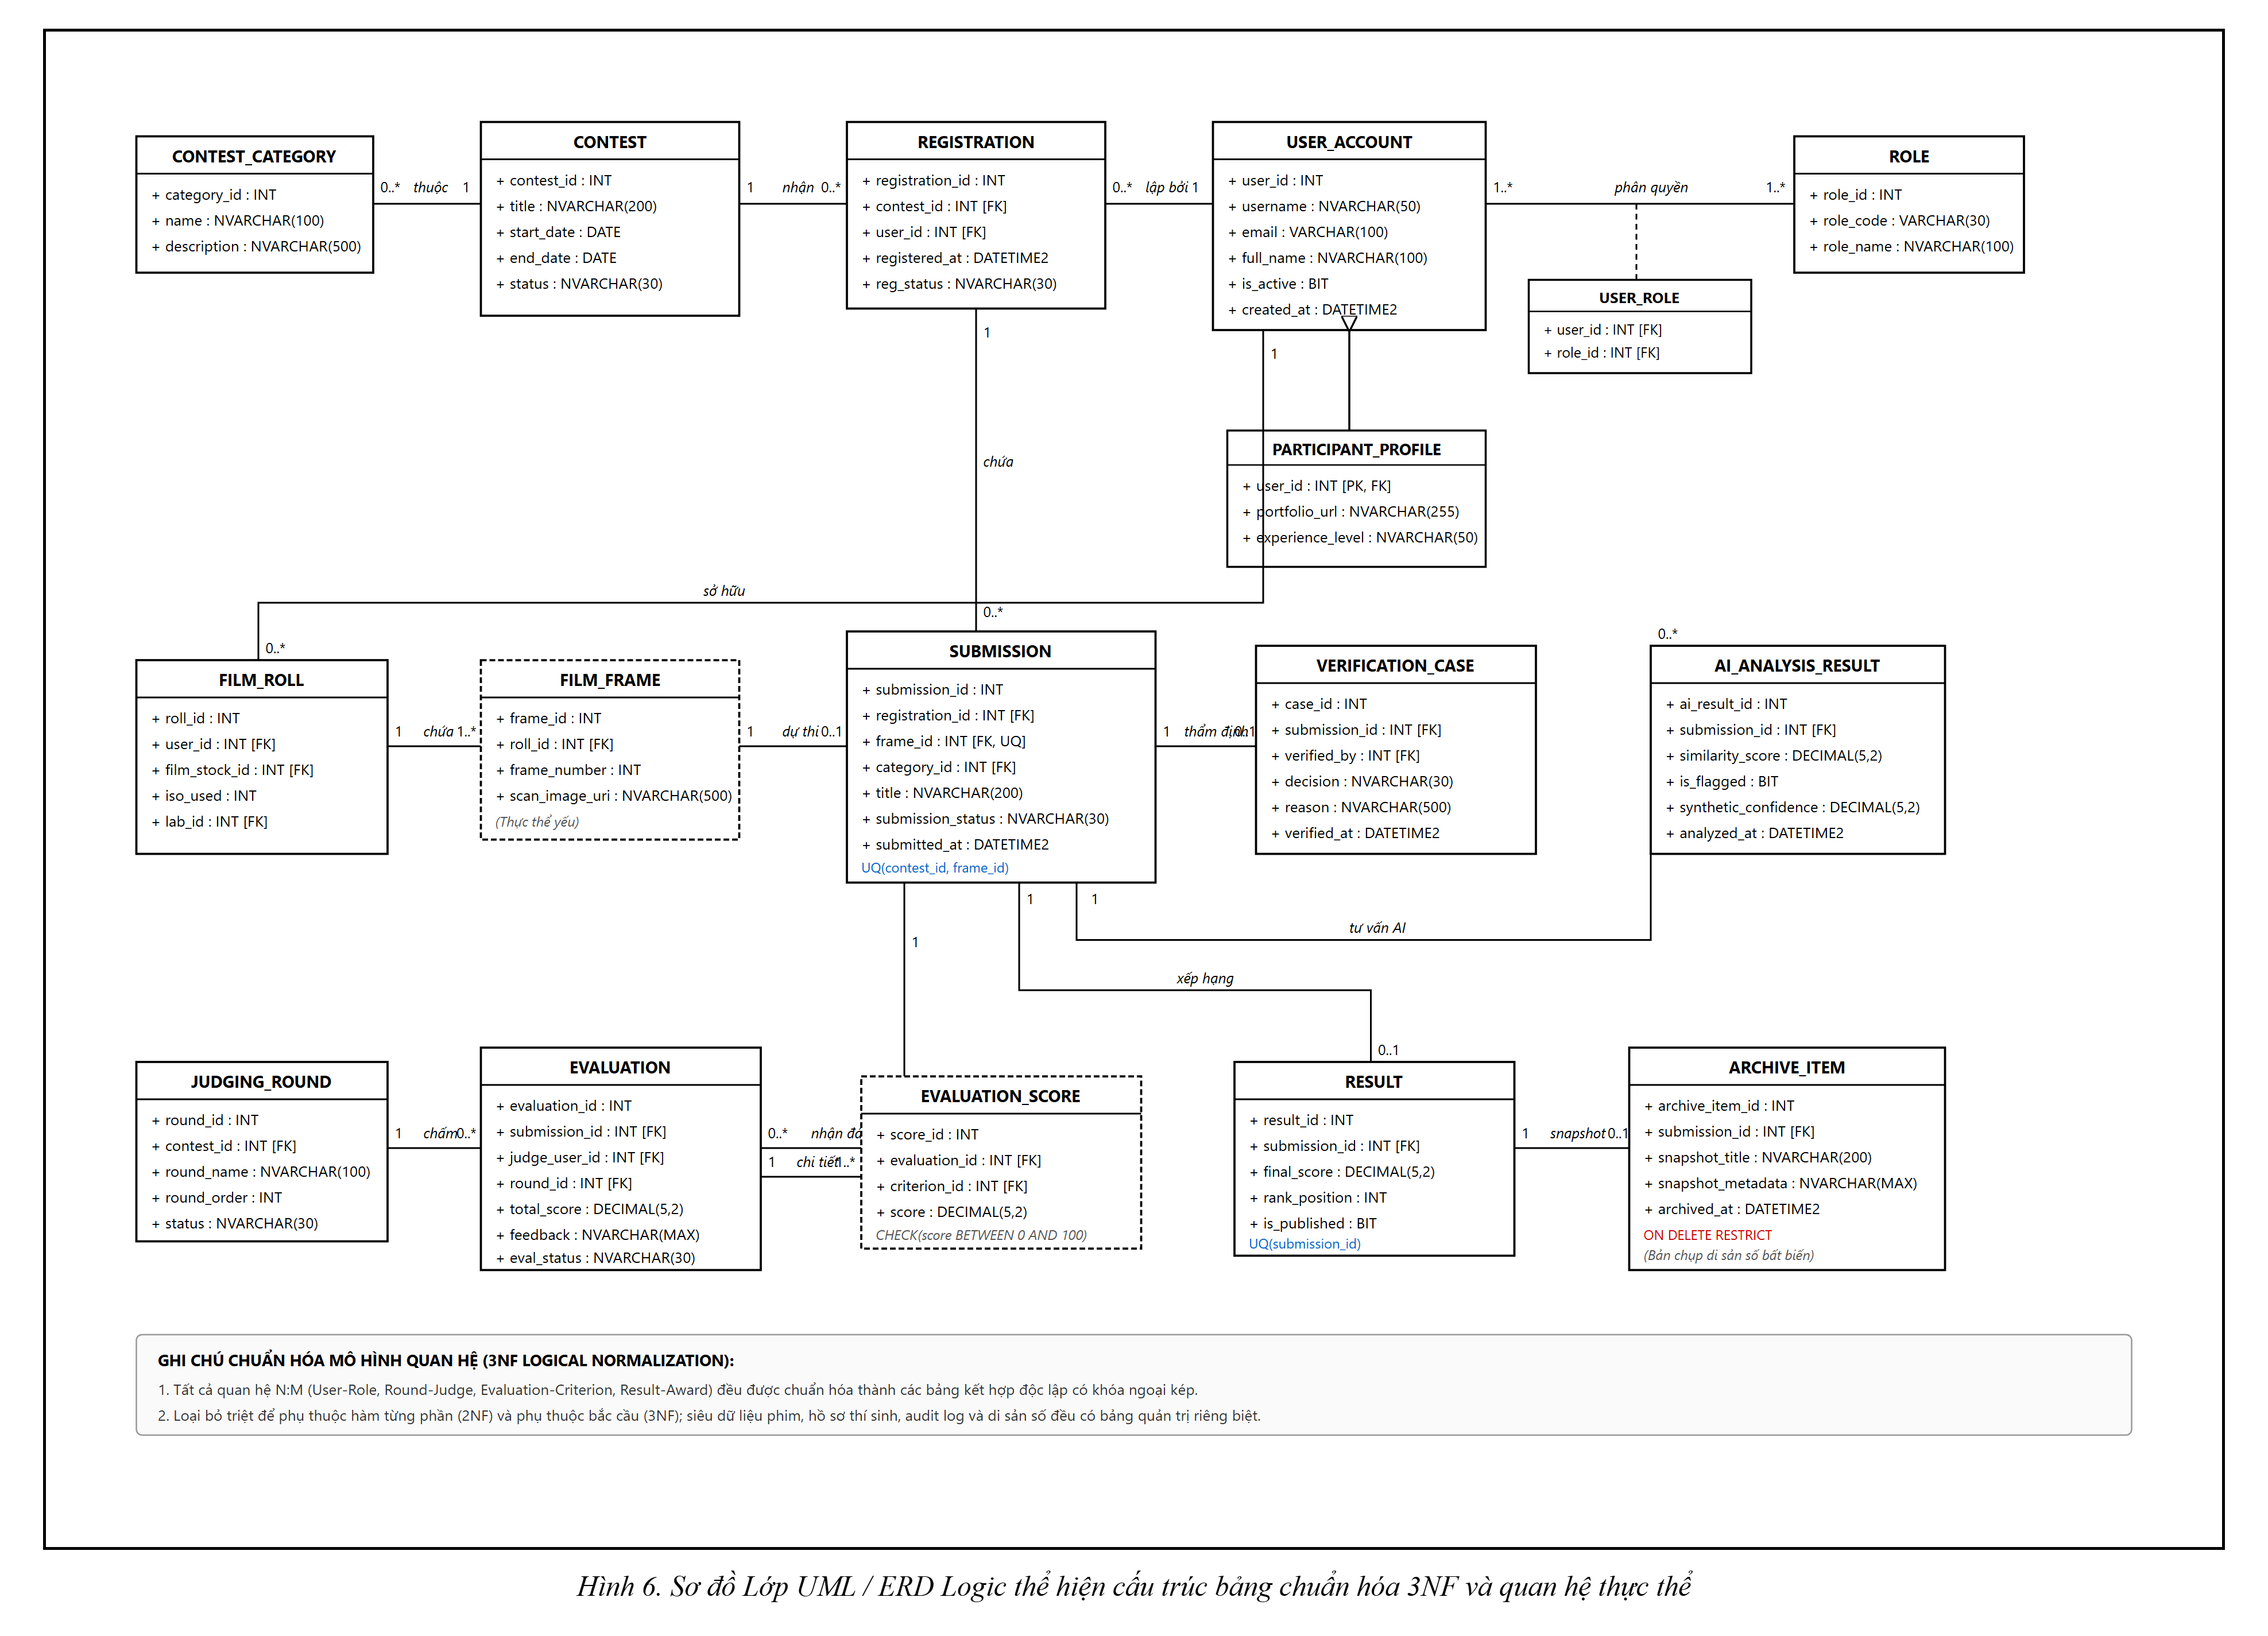
\includegraphics[width=\textwidth,keepaspectratio]{figures/fig_logical_erd.png}
    \caption{Sơ đồ Lớp / Mô hình Quan hệ Logic (Logical Schema / UML Class Diagram) đạt chuẩn 3NF}
    \label{fig:c4_logical_erd}
\end{figure}

% ----------------------------------------------------------------------
\section{Chứng minh Chuẩn hóa Dữ liệu (Normalization Proof to 3NF)}
\label{s:c4_normalization}

Để chứng minh tính đúng đắn khoa học, các quan hệ trọng yếu trong hệ thống được phân tích phụ thuộc hàm (\textit{Functional Dependencies - FD}) và chứng minh đạt dạng chuẩn 3 (3NF):

\subsection{Quan hệ FilmFrame (Khung hình phim)}
\begin{itemize}
    \item \textbf{Tập thuộc tính}: 
    \begin{center}
    $\text{FilmFrame}(\underline{\text{frame\_id}}, \text{roll\_id}, \text{camera\_id}, \text{lens\_id}, \text{frame\_number},$ \\
    $\text{frame\_title}, \text{captured\_on}, \text{capture\_location}, \text{frame\_status}, \text{negative\_uri})$
    \end{center}
    \item \textbf{Phụ thuộc hàm cốt lõi}:
    \begin{align*}
        \text{FD1: } & \text{frame\_id} \longrightarrow \{\text{roll\_id}, \text{camera\_id}, \text{lens\_id}, \\
        & \phantom{\text{frame\_id} \longrightarrow \{} \text{frame\_number}, \text{frame\_title}, \text{captured\_on}, \\
        & \phantom{\text{frame\_id} \longrightarrow \{} \text{capture\_location}, \text{frame\_status}, \text{negative\_uri}\} \\
        \text{FD2: } & (\text{roll\_id}, \text{frame\_number}) \longrightarrow \{\text{frame\_id}, \text{camera\_id}, \text{lens\_id}, \\
        & \phantom{(\text{roll\_id}, \text{frame\_number}) \longrightarrow \{} \text{frame\_title}, \text{captured\_on}, \text{capture\_location}, \\
        & \phantom{(\text{roll\_id}, \text{frame\_number}) \longrightarrow \{} \text{frame\_status}, \text{negative\_uri}\}
    \end{align*}
    \item \textbf{Chứng minh 1NF}: Mọi thuộc tính đều mang giá trị nguyên tố (\textit{atomic}), không có thuộc tính lặp hay đa trị.
    \item \textbf{Chứng minh 2NF}: Khóa chính \texttt{frame\_id} gồm 1 thuộc tính đơn lẻ, do đó không tồn tại phụ thuộc hàm bộ phận vào một phần của khóa.
    \item \textbf{Chứng minh 3NF}: Không tồn tại phụ thuộc bắc cầu giữa các thuộc tính không khóa. Thông tin về thân máy (\texttt{Camera}) và ống kính (\texttt{Lens}) đã được tách thành các quan hệ tham chiếu riêng, chỉ lưu trữ khóa ngoại tại bảng \texttt{FilmFrame}. $\Rightarrow$ \textbf{Đạt 3NF}.
\end{itemize}

\subsection{Quan hệ Submission (Bài dự thi)}
\begin{itemize}
    \item \textbf{Tập thuộc tính}: 
    \begin{center}
    $\text{Submission}(\underline{\text{submission\_id}}, \text{registration\_id}, \text{contest\_id}, \text{category\_id},$ \\
    $\text{frame\_id}, \text{submission\_title}, \text{statement}, \text{image\_uri}, \text{submitted\_at}, \text{status})$
    \end{center}
    \item \textbf{Phụ thuộc hàm cốt lõi}:
    \begin{align*}
        \text{FD1: } & \text{submission\_id} \longrightarrow \{\text{registration\_id}, \text{contest\_id}, \text{category\_id}, \\
        & \phantom{\text{submission\_id} \longrightarrow \{} \text{frame\_id}, \text{submission\_title}, \text{statement}, \\
        & \phantom{\text{submission\_id} \longrightarrow \{} \text{image\_uri}, \text{submitted\_at}, \text{status}\} \\
        \text{FD2: } & (\text{contest\_id}, \text{frame\_id}) \longrightarrow \{\text{submission\_id}, \text{registration\_id}, \\
        & \phantom{(\text{contest\_id}, \text{frame\_id}) \longrightarrow \{} \text{category\_id}, \text{submission\_title}, \\
        & \phantom{(\text{contest\_id}, \text{frame\_id}) \longrightarrow \{} \text{statement}, \text{image\_uri}, \text{submitted\_at}, \text{status}\}
    \end{align*}
    \item \textbf{Chứng minh 3NF}: Không lưu trữ lặp lại thông tin tên thí sinh hay tên cuộc thi trong bảng \texttt{Submission}. Mọi thông tin danh tính đều được truy xuất qua \texttt{registration\_id} và \texttt{frame\_id}. Không có phụ thuộc hàm giữa các thuộc tính không khóa. $\Rightarrow$ \textbf{Đạt 3NF}.
\end{itemize}

\subsection{Quan hệ EvaluationScore (Điểm tiêu chí đánh giá)}
\begin{itemize}
    \item \textbf{Tập thuộc tính}:
    \begin{center}
    $\text{EvaluationScore}(\underline{\text{evaluation\_score\_id}}, \text{evaluation\_id},$ \\
    $\text{criterion\_id}, \text{score\_value}, \text{score\_comment})$
    \end{center}
    \item \textbf{Phụ thuộc hàm cốt lõi}:
    \begin{align*}
        \text{FD1: } & \text{evaluation\_score\_id} \longrightarrow \{\text{evaluation\_id}, \text{criterion\_id}, \\
        & \phantom{\text{evaluation\_score\_id} \longrightarrow \{} \text{score\_value}, \text{score\_comment}\} \\
        \text{FD2: } & (\text{evaluation\_id}, \text{criterion\_id}) \longrightarrow \{\text{evaluation\_score\_id}, \\
        & \phantom{(\text{evaluation\_id}, \text{criterion\_id}) \longrightarrow \{} \text{score\_value}, \text{score\_comment}\}
    \end{align*}
    \item \textbf{Chứng minh 3NF}: Tên tiêu chí, thang điểm min/max và trọng số được lưu tại \texttt{ScoringCriterion}, không bị lặp lại trong \texttt{EvaluationScore}. Bảng chỉ lưu giá trị điểm và nhận xét ứng với từng tiêu chí cụ thể. $\Rightarrow$ \textbf{Đạt 3NF}.
\end{itemize}

\subsection{Quan hệ Result (Kết quả Xếp hạng và Công bố)}
\begin{itemize}
    \item \textbf{Tập thuộc tính}:
    \begin{center}
    $\text{Result}(\underline{\text{result\_id}}, \text{category\_id}, \text{submission\_id}, \text{final\_score}, \text{final\_rank},$ \\
    $\text{result\_status}, \text{tie\_break\_note}, \text{finalized\_at}, \text{finalized\_by\_user\_id}, \text{published\_at})$
    \end{center}
    \item \textbf{Phụ thuộc hàm cốt lõi}:
    \begin{align*}
        \text{FD1: } & \text{result\_id} \longrightarrow \{\text{category\_id}, \text{submission\_id}, \text{final\_score}, \text{final\_rank}, \\
        & \qquad \text{result\_status}, \text{tie\_break\_note}, \text{finalized\_at}, \\
        & \qquad \text{finalized\_by\_user\_id}, \text{published\_at}\} \\
        \text{FD2: } & (\text{category\_id}, \text{submission\_id}) \longrightarrow \{\text{result\_id}, \text{final\_score}, \text{final\_rank}, \\
        & \qquad \text{result\_status}, \text{tie\_break\_note}, \text{finalized\_at}, \\
        & \qquad \text{finalized\_by\_user\_id}, \text{published\_at}\}
    \end{align*}
    \item \textbf{Chứng minh 3NF}: Không lưu trữ lặp lại thông tin thí sinh, cuộn phim hay tên hạng mục trong bảng \texttt{Result}. Toàn bộ thông tin ngữ cảnh được truy xuất gián tiếp qua khóa ngoại \texttt{category\_id} và \texttt{submission\_id}. Ý nghĩa của kết quả phụ thuộc hàm đầy đủ vào cặp thực thể (\texttt{category\_id}, \texttt{submission\_id}). $\Rightarrow$ \textbf{Đạt 3NF}.
\end{itemize}

% ----------------------------------------------------------------------
\section{Chiến lược Phi Chuẩn hóa có Kiểm soát cho Kho Lưu trữ Số}
\label{s:c4_archive_denormalization}

Quan hệ \texttt{ArchiveItem} là trường hợp ngoại lệ duy nhất được cố tình thiết kế theo hướng \textbf{Phi chuẩn hóa có kiểm soát (\textit{Controlled Denormalization})}:

\begin{itemize}
    \item Thay vì chỉ lưu trữ các khóa ngoại sống (\texttt{result\_id}, \texttt{submission\_id}) trỏ về các bảng giao dịch, \texttt{ArchiveItem} lưu trữ các bản chụp JSON bất biến: \texttt{contest\_snapshot}, \texttt{category\_snapshot}, \texttt{participant\_snapshot}, \texttt{technical\_snapshot}, \texttt{judging\_snapshot}.
    \item \textbf{Căn cứ lý thuyết \& Thực tiễn}: Kho lưu trữ di sản số có mục đích bảo tồn nguyên trạng giá trị lịch sử tại thời điểm trao giải. Nếu trong tương lai tài khoản thí sinh đổi tên, hoặc cấu hình cuộc thi gốc bị điều chỉnh/ẩn đi, tác phẩm trong kho lưu trữ di sản vẫn giữ nguyên 100\% thông tin trung thực của thời điểm đoạt giải mà không bị sai lệch.
\end{itemize}

% ----------------------------------------------------------------------
\section{Từ điển Dữ liệu Logic (Logical Data Dictionary)}
\label{s:c4_data_dictionary}

Bảng~\ref{tab:c4_data_dictionary} hệ thống hóa từ điển dữ liệu logic cho các thuộc tính nghiệp vụ cốt lõi, xác lập rõ ranh giới ngữ nghĩa và vòng đời dữ liệu giữa các phân hệ:

\begin{table}[!ht]
\centering
\caption{Từ điển dữ liệu logic cho các thực thể và thuộc tính trọng yếu}
\label{tab:c4_data_dictionary}
\footnotesize
\begin{tabularx}{\textwidth}{>{\bfseries\raggedright\arraybackslash}p{4.2cm}>{\raggedright\arraybackslash}X>{\raggedright\arraybackslash}p{2.8cm}}
\toprule
\textbf{Thực thể.Thuộc tính} & \textbf{Ý nghĩa nghiệp vụ \& Ràng buộc logic} & \textbf{Miền giá trị / Quy ước} \\
\midrule
UserAccount.\allowbreak email & Địa chỉ email duy nhất dùng đăng nhập hệ thống & Duy nhất (UNIQUE), hợp lệ \\
Role.\allowbreak role\_code & Mã vai trò kiểm soát truy cập (RBAC) & ADMIN, ORGANIZER, \allowbreak JUDGE, PARTICIPANT \\
ParticipantProfile.\allowbreak status & Trạng thái hoạt động của hồ sơ thí sinh & ACTIVE, INACTIVE, \allowbreak SUSPENDED \\
Contest.\allowbreak contest\_code & Mã định danh nghiệp vụ của cuộc thi & Duy nhất toàn hệ thống \\
Contest.\allowbreak contest\_status & Vòng đời tổ chức của cuộc thi & DRAFT, PUBLISHED, \allowbreak OPEN, CLOSED, \allowbreak FINALIZED, ARCHIVED \\
ContestCategory.\allowbreak category\_code & Mã hạng mục chuyên môn trong cuộc thi & Duy nhất trong phạm vi contest \\
JudgingRound.\allowbreak is\_final\_round & Cờ đánh dấu vòng chấm chung khảo quyết định giải & TRUE / FALSE \\
ScoringCriterion.\allowbreak weight\_percent & Trọng số đóng góp của tiêu chí vào điểm tổng & $0 < \text{weight} \leq 100$ \\
FilmFrame.\allowbreak frame\_number & Số thứ tự khung hình trên cuộn phim vật lý & Duy nhất theo từng roll\_id \\
Submission.\allowbreak submission\_status & Trạng thái xử lý bài thi qua các giai đoạn & PENDING\_VERIFICATION, \allowbreak VERIFIED, REJECTED, \allowbreak JUDGED, FINALIZED \\
VerificationCase.\allowbreak final\_decision & Quyết định thẩm định chính thức của con người & VERIFIED, REJECTED, \allowbreak NEEDS\_CLARIFICATION \\
AIAnalysisResult.\allowbreak confidence & Điểm số tin cậy do mô hình AI trả về & $0.0000 \leq \text{conf} \leq 1.0000$ \\
JudgeAssignment.\allowbreak status & Tình trạng nhận việc của giám khảo trong vòng & ASSIGNED, IN\_PROGRESS, \allowbreak SUBMITTED, CANCELLED \\
Evaluation.\allowbreak total\_score & Tổng điểm có trọng số của một giám khảo & Tổng điểm hợp lệ $\geq 0$ \\
Result.\allowbreak final\_rank & Thứ hạng chung cuộc của bài thi trong hạng mục & Số nguyên dương $\geq 1$ \\
ArchiveItem.\allowbreak contest\_snapshot & Bản chụp bất biến của cuộc thi tại thời điểm trao giải & Định dạng JSON cấu trúc \\
AuditLog.\allowbreak action\_code & Mã định danh hành động nghiệp vụ cần kiểm toán & INSERT, UPDATE, \allowbreak STATUS\_CHANGE \\
ContestTemplate.\allowbreak template\_code & Mã định danh duy nhất của mẫu cấu hình cuộc thi & Duy nhất (UNIQUE), hợp lệ \\
AssetMetadata.\allowbreak checksum\_sha256 & Mã băm SHA-256 64 ký tự hex kiểm tra toàn vẹn tệp & Đúng 64 ký tự hex hợp lệ \\
AssetMetadata.\allowbreak qc\_status & Kết quả kiểm tra chất lượng số hóa tệp ảnh scan & PASSED, FAILED, \allowbreak FLAGGED, PENDING \\
\bottomrule
\end{tabularx}
\end{table}

% ----------------------------------------------------------------------
\section{Vòng đời Trạng thái của các Thực thể Cốt lõi (Entity Lifecycle)}
\label{s:c4_lifecycles}

Sự vận hành của cơ sở dữ liệu được định hướng bởi các máy trạng thái hữu hạn (\textit{Finite State Machines}) chặt chẽ. Bảng~\ref{tab:c4_lifecycles} tổng kết chuỗi chuyển đổi trạng thái hợp lệ của các thực thể trung tâm:

\begin{table}[!ht]
\centering
\caption{Tổng hợp vòng đời trạng thái của các thực thể cốt lõi trong hệ thống}
\label{tab:c4_lifecycles}
\small
\begin{tabularx}{\textwidth}{>{\bfseries}p{3.2cm}>{\raggedright\arraybackslash}X}
\toprule
\textbf{Thực thể} & \textbf{Chuỗi chuyển đổi trạng thái vòng đời chuẩn} \\
\midrule
Contest & \texttt{DRAFT} $\rightarrow$ \texttt{PUBLISHED} $\rightarrow$ \texttt{OPEN} $\rightarrow$ \texttt{CLOSED} $\rightarrow$ \texttt{FINALIZED} $\rightarrow$ \texttt{ARCHIVED} \\
Registration & \texttt{PENDING} $\rightarrow$ \texttt{APPROVED} / \texttt{REJECTED} / \texttt{WITHDRAWN} \\
FilmRoll & \texttt{DRAFT} $\rightarrow$ \texttt{READY} $\rightarrow$ \texttt{ARCHIVED} \\
FilmFrame & \texttt{DRAFT} $\rightarrow$ \texttt{READY} $\rightarrow$ \texttt{SUBMITTED} $\rightarrow$ \texttt{ARCHIVED} \\
Submission & \texttt{DRAFT} $\rightarrow$ \texttt{PENDING\_VERIFICATION} $\rightarrow$ \texttt{VERIFIED} / \texttt{REJECTED} / \\
 & \texttt{NEEDS\_CLARIFICATION} $\rightarrow$ \texttt{JUDGED} $\rightarrow$ \texttt{FINALIZED} $\rightarrow$ \texttt{ARCHIVED} \\
VerificationCase & \texttt{PENDING} $\rightarrow$ \texttt{UNDER\_REVIEW} $\rightarrow$ \texttt{VERIFIED} / \texttt{REJECTED} / \texttt{NEEDS\_CLARIFICATION} \\
JudgeAssignment & \texttt{ASSIGNED} $\rightarrow$ \texttt{IN\_PROGRESS} $\rightarrow$ \texttt{SUBMITTED} / \texttt{CANCELLED} \\
Evaluation & \texttt{DRAFT} $\rightarrow$ \texttt{SUBMITTED} $\rightarrow$ \texttt{LOCKED} \\
Result & \texttt{DRAFT} $\rightarrow$ \texttt{FINALIZED} $\rightarrow$ \texttt{PUBLISHED} \\
ArchiveItem & \texttt{PENDING\_ARCHIVE} $\rightarrow$ \texttt{ARCHIVED} $\rightarrow$ \texttt{RETIRED} \\
\bottomrule
\end{tabularx}
\end{table}
